%%%%%%%%%%%%%%%%%%%%%%%%%%%%%%%%%%%%%%%%%
% Masters/Doctoral Thesis 
% LaTeX Template
% Version 2.5 (27/8/17)
%
% This template was downloaded from:
% http://www.LaTeXTemplates.com
%
% Version 2.x major modifications by:
% Vel (vel@latextemplates.com)
%
% This template is based on a template by:
% Steve Gunn (http://users.ecs.soton.ac.uk/srg/softwaretools/document/templates/)
% Sunil Patel (http://www.sunilpatel.co.uk/thesis-template/)
%
% Template license:
% CC BY-NC-SA 3.0 (http://creativecommons.org/licenses/by-nc-sa/3.0/)
%
%%%%%%%%%%%%%%%%%%%%%%%%%%%%%%%%%%%%%%%%%

%----------------------------------------------------------------------------------------
%	PACKAGES AND OTHER DOCUMENT CONFIGURATIONS
%----------------------------------------------------------------------------------------

\documentclass[
11pt, % The default document font size, options: 10pt, 11pt, 12pt
%oneside, % Two side (alternating margins) for binding by default, uncomment to switch to one side
spanish, % ngerman for German
singlespacing, % Single line spacing, alternatives: onehalfspacing or doublespacing
%draft, % Uncomment to enable draft mode (no pictures, no links, overfull hboxes indicated)
%nolistspacing, % If the document is onehalfspacing or doublespacing, uncomment this to set spacing in lists to single
%liststotoc, % Uncomment to add the list of figures/tables/etc to the table of contents
%toctotoc, % Uncomment to add the main table of contents to the table of contents
%parskip, % Uncomment to add space between paragraphs
%nohyperref, % Uncomment to not load the hyperref package
headsepline, % Uncomment to get a line under the header
%chapterinoneline, % Uncomment to place the chapter title next to the number on one line
%consistentlayout, % Uncomment to change the layout of the declaration, abstract and acknowledgements pages to match the default layout
]{MastersDoctoralThesis} % The class file specifying the document structure

\usepackage[utf8]{inputenc} % Required for inputting international characters
\usepackage[T1]{fontenc} % Output font encoding for international characters

%\usepackage{mathpazo} % Use the Palatino font by default

\usepackage[backend=bibtex,style=chem-acs, natbib=true]{biblatex} % Use the bibtex backend with the authoryear citation style (which resembles APA)

\addbibresource{example.bib} % The filename of the bibliography

\usepackage[autostyle=true]{csquotes} % Required to generate language-dependent quotes in the bibliography

\renewcommand{\thesection}{\arabic{section}}

\usepackage{multirow}

%----------------------------------------------------------------------------------------
%	MARGIN SETTINGS
%----------------------------------------------------------------------------------------

\geometry{
	paper=letterpaper, % Change to letterpaper for US letter
	inner=2.5cm, % Inner margin
	outer=2.5cm, % Outer margin
	bindingoffset=.5cm, % Binding offset
	top=1.5cm, % Top margin
	bottom=1.5cm, % Bottom margin
	%showframe, % Uncomment to show how the type block is set on the page
}

%----------------------------------------------------------------------------------------
%	THESIS INFORMATION
%----------------------------------------------------------------------------------------

\thesistitle{Thesis Title} % Your thesis title, this is used in the title and abstract, print it elsewhere with \ttitle
\supervisor{Dr. Edgar Francisco \textsc{Vargas}} % Your supervisor's name, this is used in the title page, print it elsewhere with \supname
\examiner{} % Your examiner's name, this is not currently used anywhere in the template, print it elsewhere with \examname
\degree{Propuesta Proyecto de Grado } % Your degree name, this is used in the title page and abstract, print it elsewhere with \degreename
\author{Juan \textsc{Barbosa}} % Your name, this is used in the title page and abstract, print it elsewhere with \authorname
\addresses{} % Your address, this is not currently used anywhere in the template, print it elsewhere with \addressname

\subject{Química} % Your subject area, this is not currently used anywhere in the template, print it elsewhere with \subjectname
\keywords{} % Keywords for your thesis, this is not currently used anywhere in the template, print it elsewhere with \keywordnames
\university{\href{http://www.uniandes.edu.co}{Universidad de los Andes}} % Your university's name and URL, this is used in the title page and abstract, print it elsewhere with \univname
\department{\href{http://quimica.uniandes.edu.co}{Departamento de Química}} % Your department's name and URL, this is used in the title page and abstract, print it elsewhere with \deptname
\group{\href{http://quimica.uniandes.edu.co}{Termodinámica de Soluciones}} % Your research group's name and URL, this is used in the title page, print it elsewhere with \groupname
\faculty{\href{http://ciencias.uniandes.com}{Facultad de Ciencias}} % Your faculty's name and URL, this is used in the title page and abstract, print it elsewhere with \facname

\AtBeginDocument{
\hypersetup{pdftitle=\ttitle} % Set the PDF's title to your title
\hypersetup{pdfauthor=\authorname} % Set the PDF's author to your name
\hypersetup{pdfkeywords=\keywordnames} % Set the PDF's keywords to your keywords
}

\begin{document}

\frontmatter % Use roman page numbering style (i, ii, iii, iv...) for the pre-content pages

\pagestyle{plain} % Default to the plain heading style until the thesis style is called for the body content

%----------------------------------------------------------------------------------------
%	TITLE PAGE
%----------------------------------------------------------------------------------------

\begin{titlepage}
\begin{center}

\vspace*{.06\textheight}
{\scshape\LARGE \univname\par}\vspace{1.5cm} % University name
\textsc{\Large Propuesta de Grado}\\[0.5cm] % Thesis type

\HRule \\[0.4cm] % Horizontal line
{\huge \bfseries \ttitle\par}\vspace{0.4cm} % Thesis title
\HRule \\[1.5cm] % Horizontal line
 
\begin{minipage}[t]{0.4\textwidth}
\begin{flushleft} \large
\emph{Autor:}\\
\href{https://www.github.com/jsbarbosa}{\authorname} % Author name - remove the \href bracket to remove the link
\end{flushleft}
\end{minipage}
\begin{minipage}[t]{0.4\textwidth}
\begin{flushright} \large
\emph{Director:} \\
\href{http://quimica.uniandes.edu.co/es/el-departamento/profesores/planta-3#}{\supname} % Supervisor name - remove the \href bracket to remove the link  
\end{flushright}
\end{minipage}\\[3cm]
 
\vfill

\large \textit{\degreename para optar por el título de Químico}\\[0.3cm] % University requirement text
%\textit{en el}\\[0.4cm]
\groupname\\\deptname\\[2cm] % Research group name and department name
 
\vfill

{\large \today}\\[4cm] % Date
%\includegraphics{Logo} % University/department logo - uncomment to place it
 
\vfill
\end{center}
\end{titlepage}

%----------------------------------------------------------------------------------------
%	DECLARATION PAGE
%----------------------------------------------------------------------------------------

%\begin{declaration}
%\addchaptertocentry{\authorshipname} % Add the declaration to the table of contents
%\noindent I, \authorname, declare that this thesis titled, \enquote{\ttitle} and the work presented in it are my own. I confirm that:
%
%\begin{itemize} 
%\item This work was done wholly or mainly while in candidature for a research degree at this University.
%\item Where any part of this thesis has previously been submitted for a degree or any other qualification at this University or any other institution, this has been clearly stated.
%\item Where I have consulted the published work of others, this is always clearly attributed.
%\item Where I have quoted from the work of others, the source is always given. With the exception of such quotations, this thesis is entirely my own work.
%\item I have acknowledged all main sources of help.
%\item Where the thesis is based on work done by myself jointly with others, I have made clear exactly what was done by others and what I have contributed myself.\\
%\end{itemize}
% 
%\noindent Signed:\\
%\rule[0.5em]{25em}{0.5pt} % This prints a line for the signature
% 
%\noindent Date:\\
%\rule[0.5em]{25em}{0.5pt} % This prints a line to write the date
%\end{declaration}

\cleardoublepage

%----------------------------------------------------------------------------------------
%	QUOTATION PAGE
%----------------------------------------------------------------------------------------

%\vspace*{0.2\textheight}
%
%\noindent\enquote{\itshape Thanks to my solid academic training, today I can write hundreds of words on virtually any topic without possessing a shred of information, which is how I got a good job in journalism.}\bigbreak
%
%\hfill Dave Barry

%----------------------------------------------------------------------------------------
%	ABSTRACT PAGE
%----------------------------------------------------------------------------------------

%\begin{abstract}
%\addchaptertocentry{\abstractname} % Add the abstract to the table of contents
%The Thesis Abstract is written here (and usually kept to just this page). The page is kept centered vertically so can expand into the blank space above the title too\ldots
%\end{abstract}

%----------------------------------------------------------------------------------------
%	ACKNOWLEDGEMENTS
%----------------------------------------------------------------------------------------

%\begin{acknowledgements}
%\addchaptertocentry{\acknowledgementname} % Add the acknowledgements to the table of contents
%The acknowledgments and the people to thank go here, don't forget to include your project advisor\ldots
%\end{acknowledgements}

%----------------------------------------------------------------------------------------
%	LIST OF CONTENTS/FIGURES/TABLES PAGES
%----------------------------------------------------------------------------------------
%
%\tableofcontents % Prints the main table of contents
%
%\listoffigures % Prints the list of figures
%
%\listoftables % Prints the list of tables

%----------------------------------------------------------------------------------------
%	ABBREVIATIONS
%----------------------------------------------------------------------------------------
%
%\begin{abbreviations}{ll} % Include a list of abbreviations (a table of two columns)
%
%\textbf{LAH} & \textbf{L}ist \textbf{A}bbreviations \textbf{H}ere\\
%\textbf{WSF} & \textbf{W}hat (it) \textbf{S}tands \textbf{F}or\\
%
%\end{abbreviations}

%----------------------------------------------------------------------------------------
%	PHYSICAL CONSTANTS/OTHER DEFINITIONS
%----------------------------------------------------------------------------------------
%
%\begin{constants}{lr@{${}={}$}l} % The list of physical constants is a three column table
%
%% The \SI{}{} command is provided by the siunitx package, see its documentation for instructions on how to use it
%
%Speed of Light & $c_{0}$ & \SI{2.99792458e8}{\meter\per\second} (exact)\\
%%Constant Name & $Symbol$ & $Constant Value$ with units\\
%
%\end{constants}

%----------------------------------------------------------------------------------------
%	SYMBOLS
%----------------------------------------------------------------------------------------

%\begin{symbols}{lll} % Include a list of Symbols (a three column table)
%
%$a$ & distance & \si{\meter} \\
%$P$ & power & \si{\watt} (\si{\joule\per\second}) \\
%%Symbol & Name & Unit \\
%
%\addlinespace % Gap to separate the Roman symbols from the Greek
%
%$\omega$ & angular frequency & \si{\radian} \\
%
%\end{symbols}

%----------------------------------------------------------------------------------------
%	DEDICATION
%----------------------------------------------------------------------------------------

%\dedicatory{For/Dedicated to/To my\ldots} 

%----------------------------------------------------------------------------------------
%	THESIS CONTENT - CHAPTERS
%----------------------------------------------------------------------------------------

\mainmatter % Begin numeric (1,2,3...) page numbering

\pagestyle{thesis} % Return the page headers back to the "thesis" style

% Include the chapters of the thesis as separate files from the Chapters folder
% Uncomment the lines as you write the chapters

% !TeX spellcheck = es_ANY
% Chapter 1

%\chapter{Chapter Title Here} % Main chapter title
%
%\label{Chapter1} % For referencing the chapter elsewhere, use \ref{Chapter1} 

%----------------------------------------------------------------------------------------

% Define some commands to keep the formatting separated from the content 
\newcommand{\keyword}[1]{\textit{#1}}
%\newcommand{\tabhead}[1]{\textbf{#1}}
%\newcommand{\code}[1]{\texttt{#1}}
%\newcommand{\file}[1]{\texttt{\bfseries#1}}
%\newcommand{\option}[1]{\texttt{\itshape#1}}

%----------------------------------------------------------------------------------------

\chapter{Introducción}
	La termodinámica es el estudio de las transformaciones de energía. En la etapa más temprana de esta rama de las ciencias, se pensaba que el calor era una clase de fluido cuya cantidad neta en el universo permanecía siempre constante. El aumento de temperatura de un cuerpo era explicado a partir de la migración de calor de un objeto a otro \cite{feynman2011feynman, fermi1986}. Usando dicha teoría del calor como fluido, el ingeniero Sadi Carnot dio origen a la termodinámica con el análisis del problema, sobre cómo generar el mejor y más eficiente motor de vapor en 1824. Posteriormente, Julius von Mayer en 1842 descubrió una equivalencia entre el calor y el trabajo mecánico, relaci\'on también publicada por James Joule el siguiente año \cite{fermi1986}. A raíz de esto hoy se considera el calor como una forma de transferencia de energía \cite{fermi1986}.
	
	Los resultados de la termodinámica se encuentran implícitos en una serie de declaraciones que reciben el nombre de leyes de la termodinámica, las cuales, en conjunto, nos permiten conocer la dirección natural en la que tienen lugar los cambios químicos y físicos en la materia \cite{atkins2011physical}. Históricamente la termodinámica fue desarrollada antes que se tuviera un entendimiento sobre la estructura interna de la materia, además, sus leyes tampoco siguen un orden cronológico \cite{feynman2011feynman}. La primera ley surge del trabajo realizado por Mayer en 1842, una de las leyes más importantes de la ciencia en general: la conservación de la energía \cite{feynman2011feynman, fermi1986}. La segunda, se atribuye a Carnot y Clausius en 1824, y habla sobre la reversibilidad o direccionalidad de los procesos \cite{feynman2011feynman}.
	
	A pesar que el estudio de las transformaciones de energía parece un tema distante de la química, la termodinámica, estudiada a través de la fisicoquímica, ha demostrado ser de vital importancia tanto en la química como la biología \cite{atkins2011physical}. No sólo permite entender la producción o consumo de energía en las reacciones químicas, sino que, constituye una herramienta fundamental para responder preguntas que se encuentran en el corazón de la bioquímica, por ejemplo sobre cómo fluye la energía en una célula, y qué tan grande puede ser la agrupación de moléculas que forman estructuras complejas como las células \cite{atkins2011physical}. En otros casos, por ejemplo, existen propiedades de fácil determinación para un analista, como el color, masa y densidad. Sin embargo, hay propiedades que dependen de los enlaces, estructura molecular y naturaleza del material, entre estas se encuentran propiedades termodinámicas de interés químico, como lo son: la capacidad calorífica, entalpía, entropía, etc \cite{gaisford2016principles}.
	
	Dentro de la fisicoquímica, el estudio y medición de la transferencia de energía en forma de calor se denomina calorimetría, y constituye una de las áreas más antiguas de esta rama de la química \cite{zielenkiewicz2006theory}. Se podría considerar que la historia de esta comienza en junio de 1783, con la presentación de \textit{Memoria del calor} (Mémoire de la Chaleur) por Lavoisier y Laplace en la Academia Francesa \cite{zielenkiewicz2006theory}. La mayoría de los procesos físicos y químicos están acompañados de absorción o liberación de energía. Lo anterior hace de la calorimetría una técnica con un amplio rango de aplicaciones \cite{wadso2001standards}. Entre estas aplicaciones se encuentran titulaciones, flujos, reacciones y estudio de procesos de sorción \cite{gaisford2016principles}.
		
	El instrumento para realizar estas mediciones se denomina calorímetro, y los hay de diversos tipos. Pueden ser clasificados por el tipo de condiciones que imponen al sistema, por ejemplo, volumen constante, temperatura constante, calor constante, etc. Estos calorímetros reciben el nombre de: bombas calorimétricas, isotérmicos, y adiabáticos, correspondientemente \cite{gaisford2016principles, wadso2001standards}. También pueden ser clasificados por el principio de funcionamiento, si compensan los flujos de energía o los acumulan \cite{gaisford2016principles}. Finalmente, dependiendo del rango de las potencias medidas, se tienen dos términos comúnmente usados: \keyword{microcalorimetría} para el caso de experimentos realizados en el rango de los microvatios \cite{wadso2001standards, wadso2003new}, mientras que para escalas de nanovatios son usados \keyword{nanocalorímetros} \cite{wadso2003new}.
	
	En particular, el trabajo que se expone en el presente documento, instal\'o, y calibr\'o un microcalorímetro 2277 Thermal Activity Monitor. Para esto fue necesario el entendimiento del funcionamiento del calorímetro a nivel interno, desde las partes hidra\'ulicas, pasando por los detalles de la electrónica hasta los principios fisicoquímicos detrás del mismo. Para confirmar que el calor\'imetro se encontraba operando de forma correcta se realizaron m\'ultiples calibraciones el\'ectricas, tanto est\'aticas como din\'amicas, las cuales resultan ser un proceso rutinario en la operaci\'on del calor\'imetro. Este calor\'imetro en particular funciona mediante el principio de transferencia de energ\'ia, en donde la diferencia de energ\'ia producida al interior de una celda de medici\'on ,fluye a trav\'es de dos elementos Peltier en un esfuerzo por establecer el equilibrio t\'ermico con los alrededores, lo cual se muestra en la \autoref{fig: heatFlow} \cite{Suurkuusk}.
	\begin{figure}[h]
		\centering
		\begin{subfigure}{0.59\linewidth}
			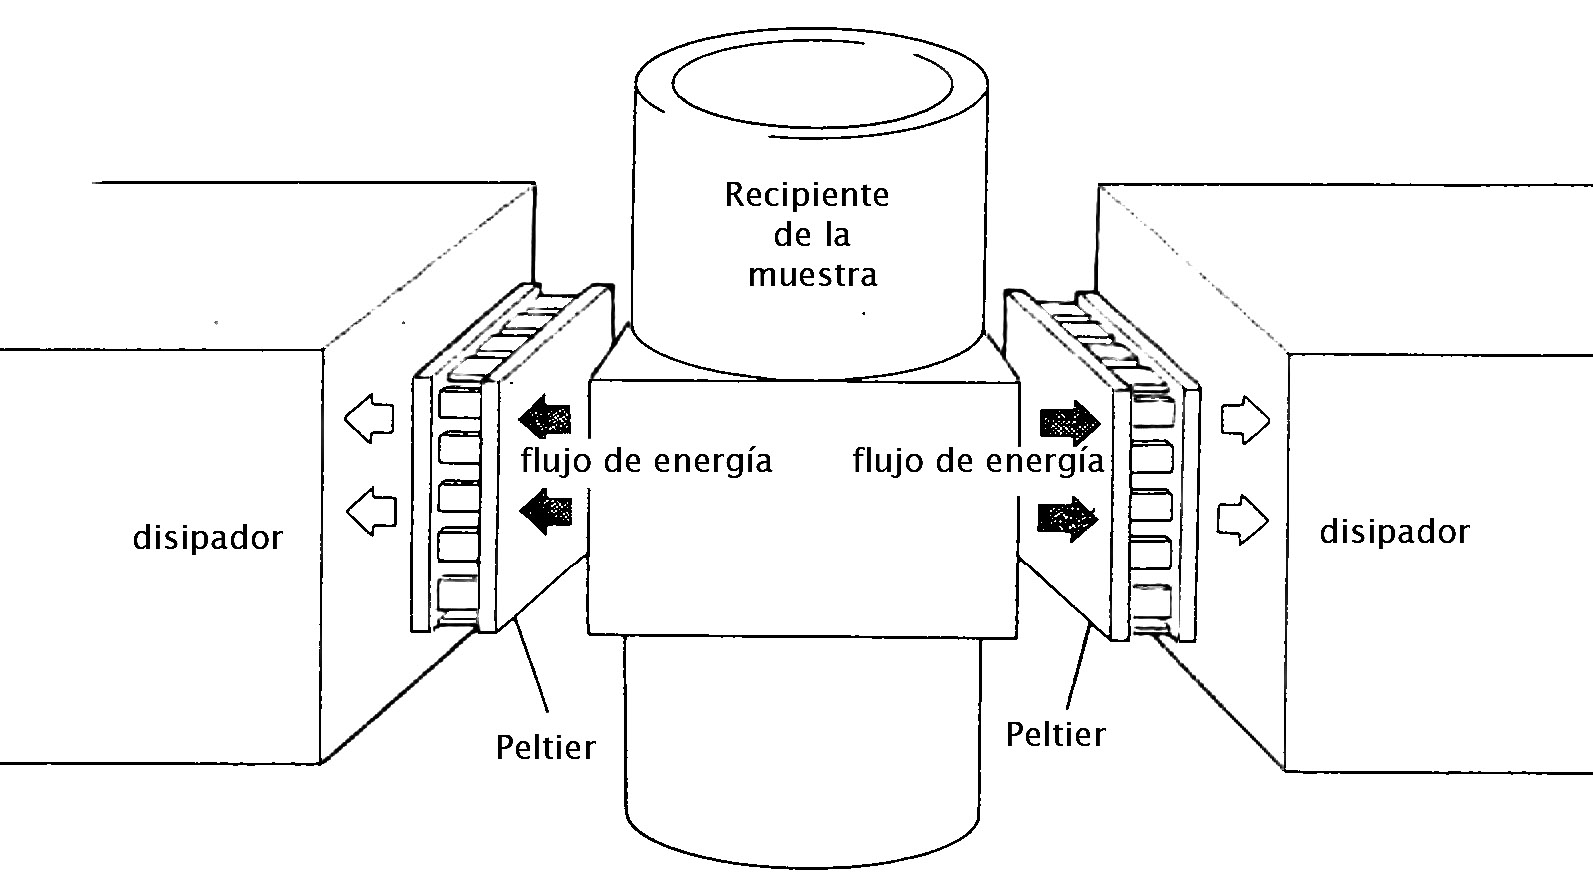
\includegraphics[width=\linewidth]{Figures/heatFlow}
			\caption{Interacci\'on de la celda de medici\'on con los alrededores, modificado de \cite{Suurkuusk}.}
			\label{fig: heatFlow}
		\end{subfigure}
		\begin{subfigure}{0.39\linewidth}
			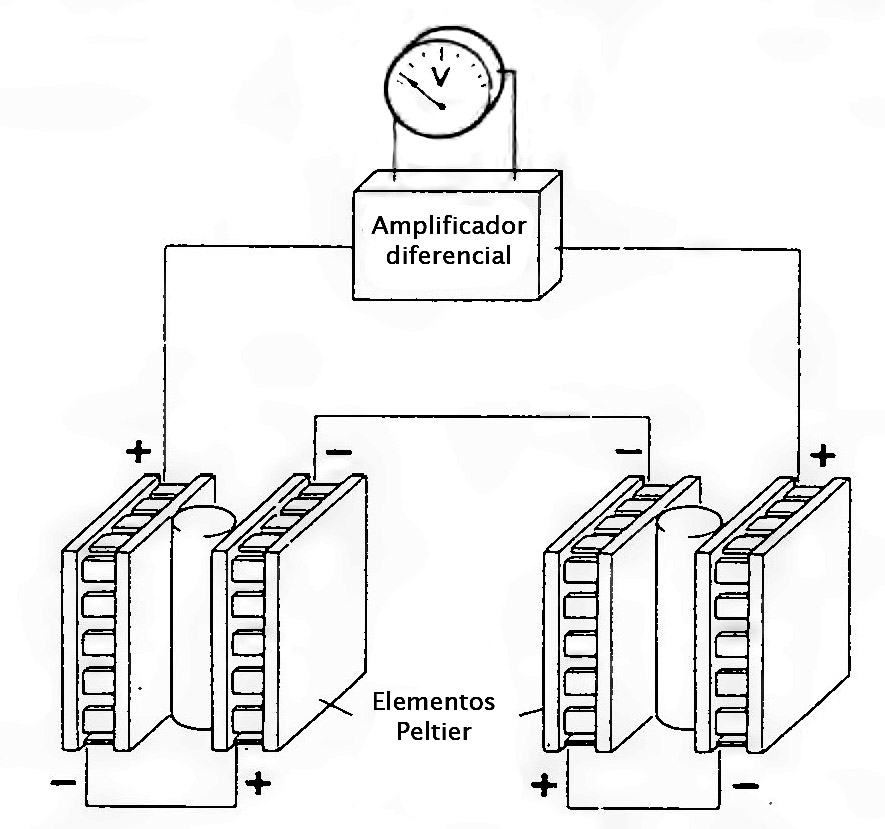
\includegraphics[width=\linewidth]{Figures/twinMeasuring}
			\caption{Principio de medici\'on de dos celdas gemelas, modificado de \cite{Suurkuusk}.}
			\label{fig: twin}
		\end{subfigure}
		\caption{Principio de detecci\'on de la energ\'ia transferida en forma de calor para cada canal de medida del calor\'imetro.}
	\end{figure}
	\newpage

	El calor\'imetro est\'a dise\~nado para que sea posible usar hasta cuatro cilindros de medici\'on independientes. Para cada uno de ellos, el principal camino del flujo de energ\'ia desde o hacia la celda es a trav\'es de los elementos Peltier \cite{Suurkuusk}. Dichos elementos est\'an compuestos de materiales semiconductores, sensibles a gradientes de temperatura del orden $1\times10^{-6}$ \grad{} \cite{Suurkuusk, simon2013oxford}. La uni\'on de estos semiconductores en serie, da lugar a detectores altamente sensibles a flujos de energ\'ia en forma de calor. Para detectar estos flujos se usa el efecto Seebeck, seg\'un el cual, para un gradiente de temperatura se genera una diferencia de potencial entre dos terminales de la celda. El efecto contrario recibe el nombre de efecto Peltier y se debe a que al pasar una corriente el\'ectrica a trav\'es de un material, se genera un transporte de energ\'ia en forma de calor. El flujo de energ\'ia t\'ermica se escribe de la siguiente forma \cite{simon2013oxford}:
	\begin{equation}\label{eq: peltier}
		\mathbf{j}^q = \Pi \mathbf{j}
	\end{equation}
	
	donde $\Pi$ recibe el nombre de coeficiente Peltier, $\mathbf{j}^q$ es la densidad de flujo de energ\'ia en forma de calor y $\mathbf{j}$ la densidad de corriente el\'ectrica \cite{simon2013oxford}. El coeficiente Seebeck ($S$) se define como $S = -\Delta V/\Delta T$ con $\Delta V$ como la diferencia de voltaje y se relaciona con el coeficiente de Peltier como: $\Pi = ST$, por lo cual al aplicar sobre la \autoref{eq: peltier} se obtiene:
	\begin{equation}\label{eq: seebeck}
		\mathbf{j}^q = (ST) \mathbf{j} = \left(-T\dfrac{\mathbf{j}}{\Delta T}\right)\Delta V = k\Delta V
	\end{equation}
	
	De esta forma se tiene que $\mathbf{j}^q \propto \Delta V$, por lo cual es posible cuantificar un flujo de energ\'ia t\'ermica en forma de calor con una lectura de potencial el\'ectrico. Las calibraciones el\'ectricas permiten determinar el valor de $k$, el cual, como se observa en la \autoref{eq: seebeck}, depende de la temperatura, por lo cual si se modifica la temperatura del ba\~no interno resulta necesario realizar una nueva calibraci\'on el\'ectrica. Dada esta dependencia con la temperatura, el calor\'imetro cuenta con un ba\~no termostatado con capacidad para 25 litros de agua, los cuales rodean los cilindros de medici\'on y act\'ua como reservorio t\'ermico \cite{Suurkuusk}. La sensibilidad a la temperatura hace que las funciones principales del calor\'imetro se encuentren divididas en dos unidades independientes, la del control de las condiciones isot\'ermicas y la detecci\'on de los eventos calorim\'etricos. La primera se encuentra descrita en el \autoref{ch: thermal}. Respecto a la segunda, la detecci\'on de los flujos de energ\'ia en forma de calor, el calor\'imetro usa dos celdas de medici\'on para cada canal de medida. Los elementos Peltier de cada canal se encuentran conectados en serie, pero con la polarizaci\'on opuesta, de tal forma que se registre la diferencia en los flujos de calor de las dos celdas, de esta forma es posible usar una para el estudio de la muestra (lado \texttt{A}) y otra para realizar un blanco (lado \texttt{B}) como se muestra en la \autoref{fig: twin}.
	 
	El calor\'imetro puede tomar medidas de ampollas, las cuales pueden ser usadas para estudiar el crecimiento de microorganismos, o en modo de titulaci\'on, para el cual es necesario contar con un agitador permanente en la soluci\'on, as\'i como de un sistema de inyecci\'on para adicionar la soluci\'on titulante \cite{Suurkuusk}. Un ejemplo de esta aplicaci\'on es la calibraci\'on qu\'imica que se muestra en el \autoref{ch: chemical}, de donde se pueden obtener propiedades termodin\'amicas del sistema a partir de la potencia registrada este. 	 

\section{Justificación del proyecto}
	En general, la calorimetría permite una gran variedad de análisis, muchos de ellos cuentan con aplicaciones industriales, comerciales, biológicos y químicos, permitiendo el entendimiento de las interacciones moleculares en soluciones \cite{blandamer1998titration}. Una ventaja de la calorimetría es que no es específica, ni invasiva, además de no depender de las propiedades electroquímicas y ópticas de un sistema dado, siendo esto de vital importancia para las investigaciones de procesos biológicos, el estudio del crecimiento bacteriano y para la detección de compuestos biológicos \cite{winkelmann2004application}. Por otro lado la calorimetría también permite el estudio de la termodinámica en sistemas de absorción, bien sea por la universalidad de la absorción física en superficies como catalizadores, o en procesos industriales como la separación de mezclas de gases \cite{morrison1987calorimetry}. Finalmente la calorimetría es el método clásico para la determinación de propiedades termodinámicas en las muestras, entre estas se encuentran: capacidad calorífica, entalpía, entropía y energía libre de Gibbs, las cuales constituyen el punto de partida de gran cantidad de estudios teóricos, desarrollos y producción industrial de un compuesto químico \cite{wang2005determination, gaisford2016principles}.
	
	El calorímetro 2277 Thermal Activity Monitor con el que cuenta el grupo de investigación, al momento de realizar este trabajo se encontraba desarmado, a la espera de su instalaci\'on y puesta en funcionamiento. Este instrumento permite monitorear una gran variedad de reacciones químicas y bioquímicas, lo anterior debido a su capacidad de cuantificar procesos exotérmicos y endotérmicos. Estas reacciones pueden ser estudiadas en el rango de 5 - 80 $^\circ$C \cite{Suurkuusk}. Este rango de temperaturas se debe al uso de un baño termostatado de 25 litros. Cuatro balones de medición independientes se encuentran sumergidos en este baño, permitiendo medidas en el rango de microvatios \cite{Suurkuusk}. Es por esta razón que poner en marcha y calibrar el equipo con el que cuenta el grupo de investigación resulta una contribución importante para el mismo, así como para el \deptname\ en general.
	
\section{Objetivos}
	\subsection{Objetivo general}
		Poner en funcionamiento el calorímetro 2277 Thermal Activity Monitor con el que se cuenta, y adicionalmente calibrar el equipo para su uso en las investigaciones activas del grupo \groupname.
		
	\subsection{Objetivos específicos}
		\begin{itemize}
			\item Realizar el cableado y conexiones electrónicas pertinentes a la instalaci\'on del equipo 2277 Thermal Activity Monitor.
			\item Mantener la temperatura del ba\~no interno estable a una temperatura de 25 \grad{}.
			\item Realizar calibraciones eléctricas, para asegurar que las señales obtenidas tengan un equivalente en potencia.
			\item Determinación de la entalpía molar, energía libre de Gibbs, entropía, y constante de afinidad, de la reacci\'on de bicarbonato de potasio con \'acido clorh\'idrico como una calibración química.
		\end{itemize}
	
	
%\section{Metodología}
%	Para el ensamble del calorímetro se cuenta con el catálogo de partes, y el manual de instrucciones. En el primero se detallan y enumeran las partes del equipo, en la \autoref{fig:partes} se muestran ejemplos de los distintos sistemas con los que el calorímetro cuenta \cite{Suurkuusk}. 
%	
%	\begin{figure}[h]
%		\centering
%		\begin{subfigure}[b]{0.3\textwidth}
%			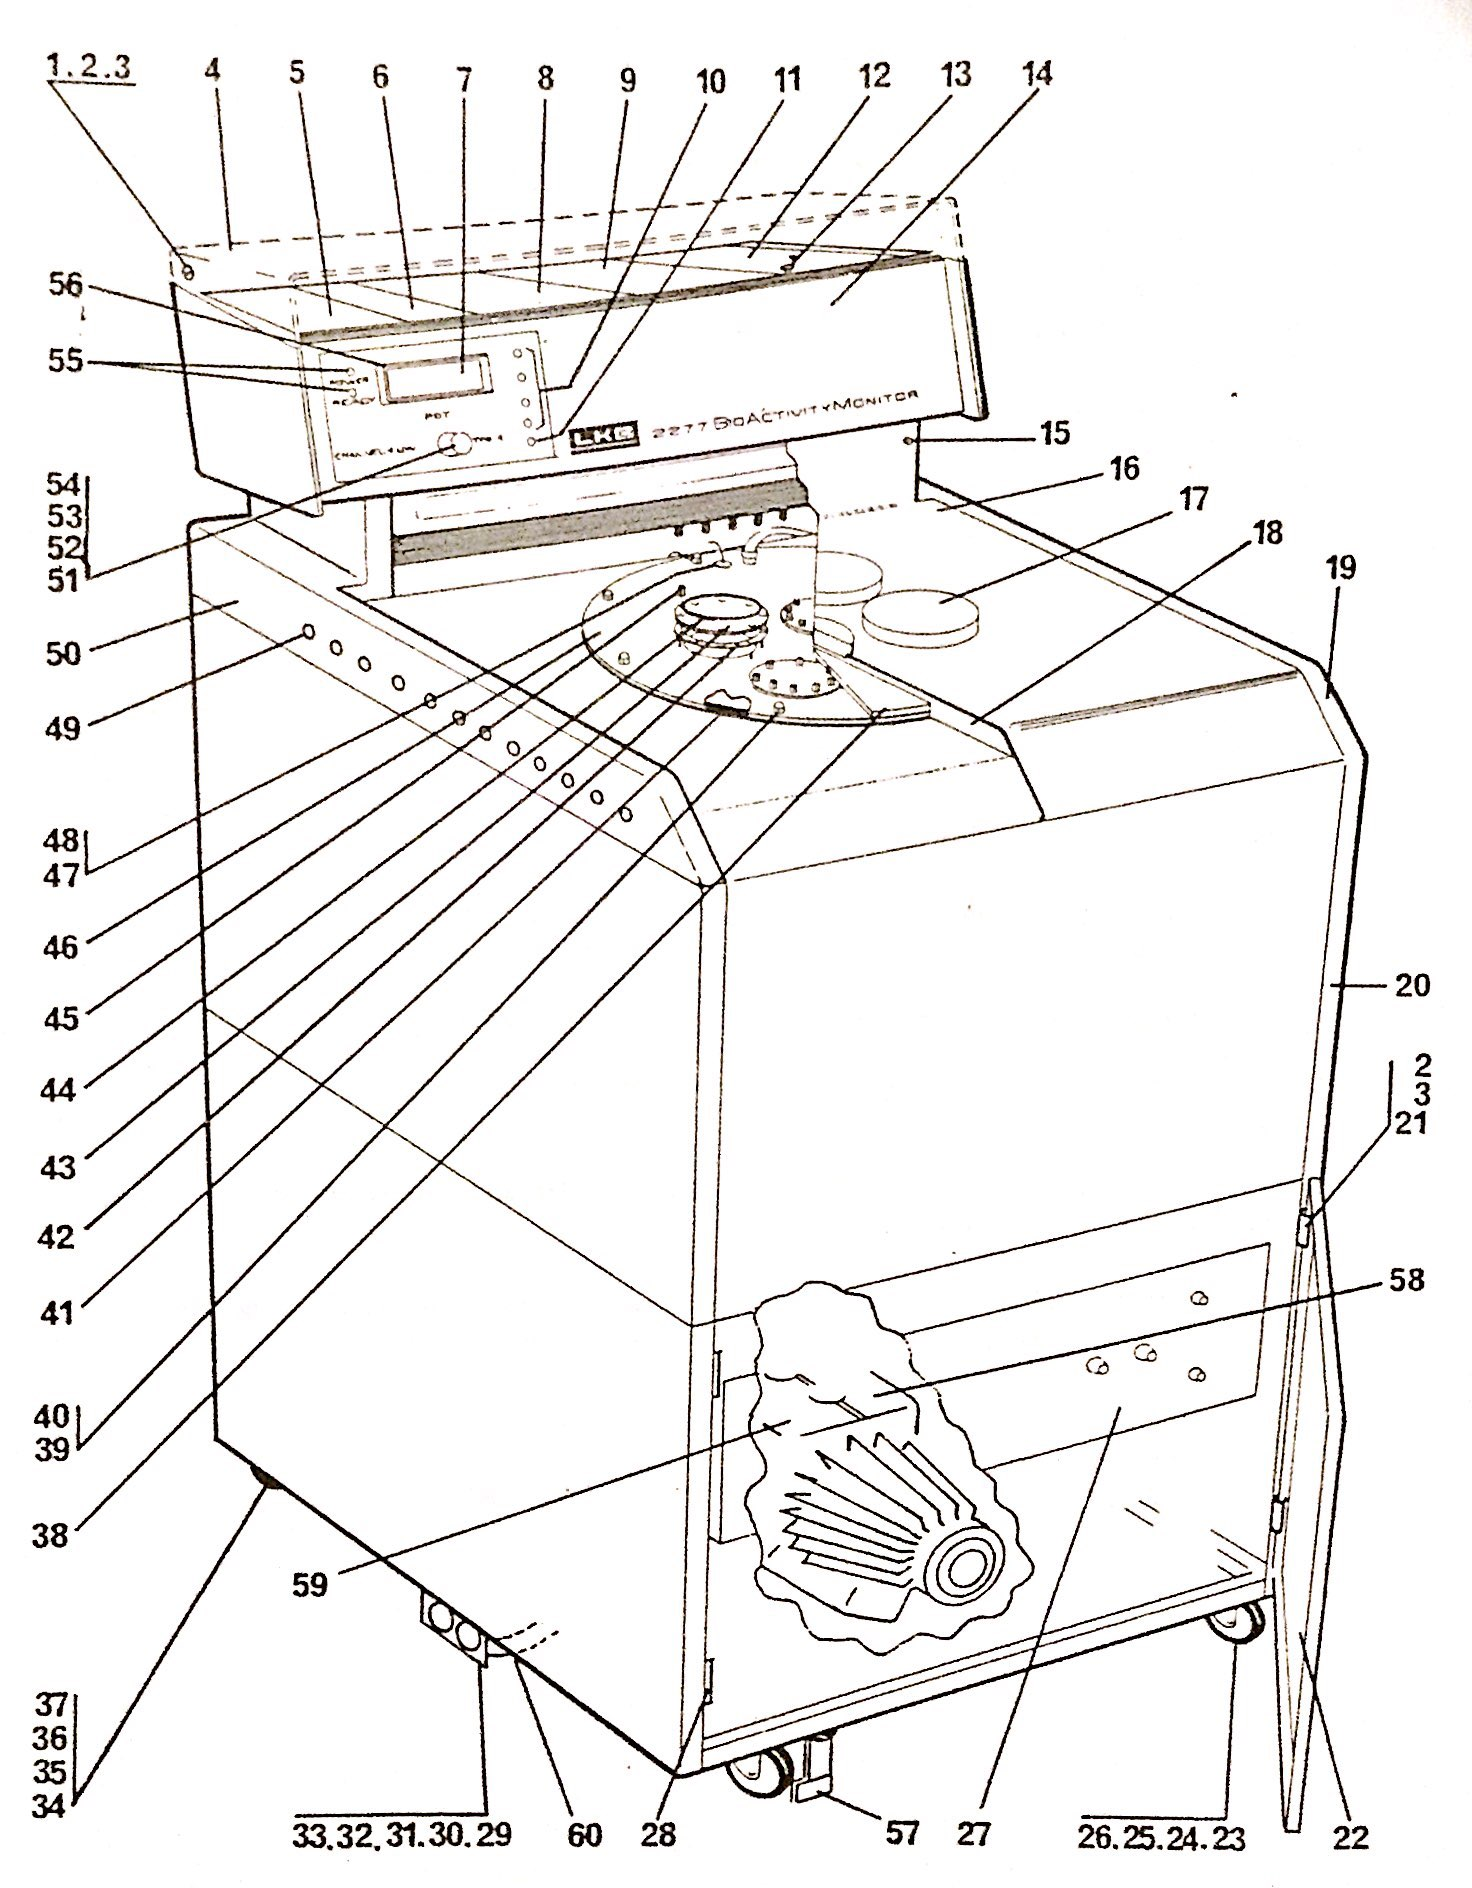
\includegraphics[width=\textwidth]{Figures/images_1.jpg}
%			\caption{Vista exterior del equipo con sus componentes.}
%			\label{fig:vistaExterior}
%		\end{subfigure}
%		~ 
%		\begin{subfigure}[b]{0.37\textwidth}
%			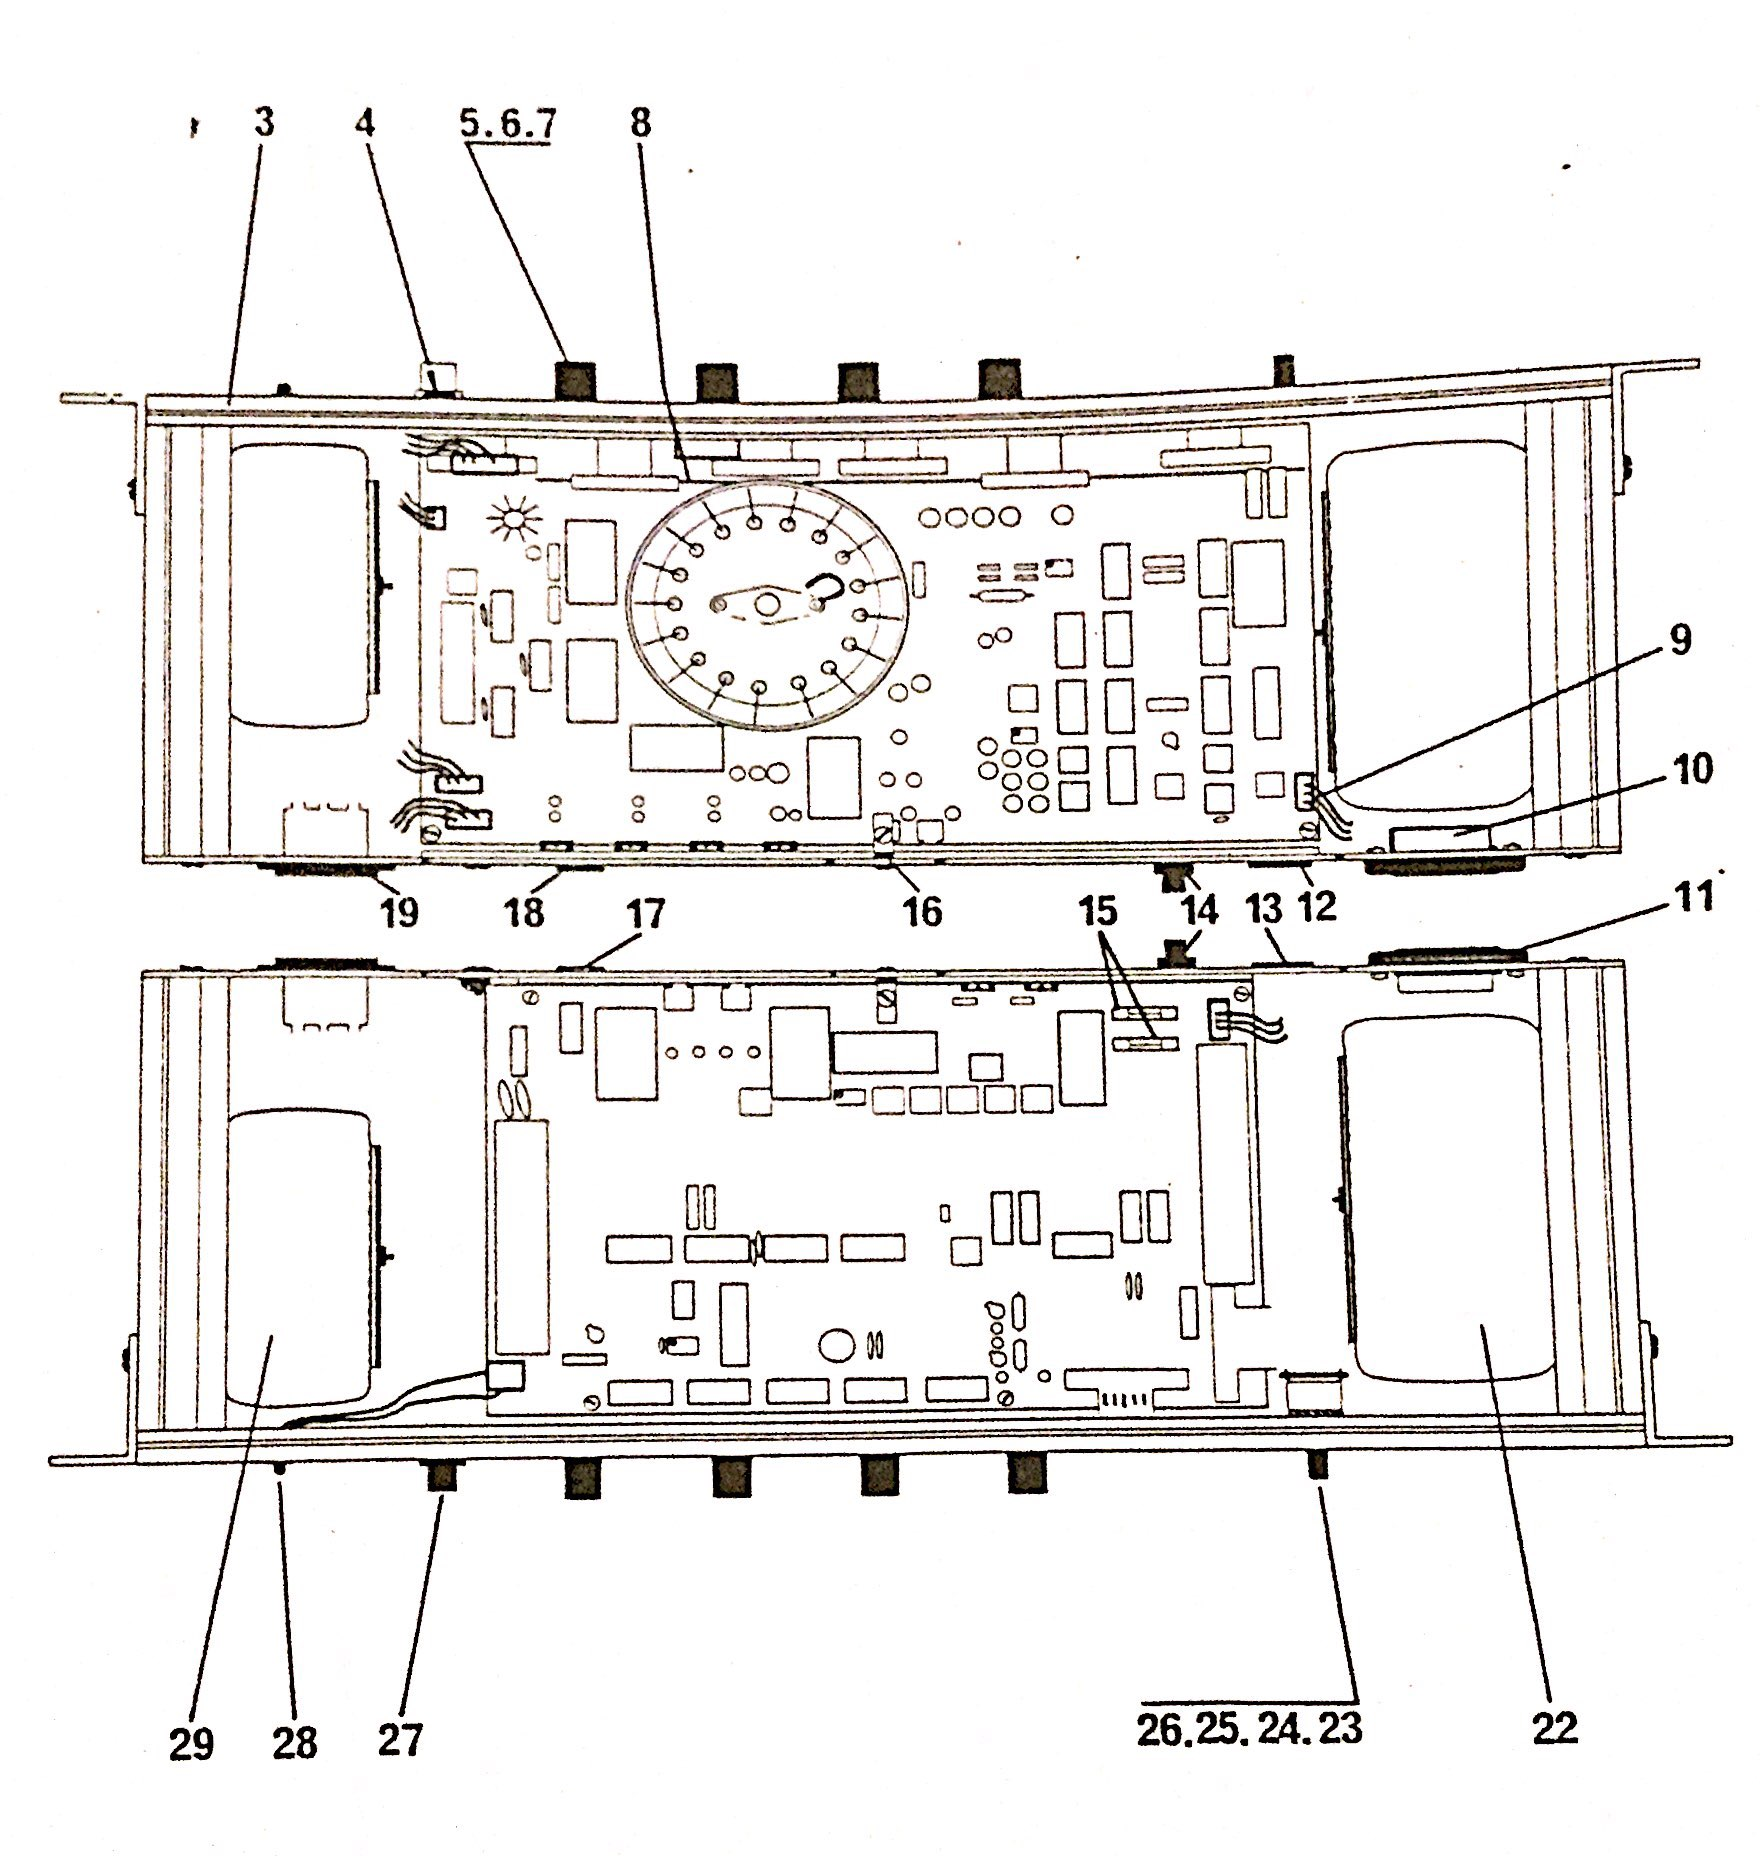
\includegraphics[width=\textwidth]{Figures/images_2.jpg}
%			\caption{Parte del sistema eléctrico del calorímetro.}
%			\label{fig:sistemaElectrico}
%		\end{subfigure}
%		~ 
%		\begin{subfigure}[b]{0.25\textwidth}
%			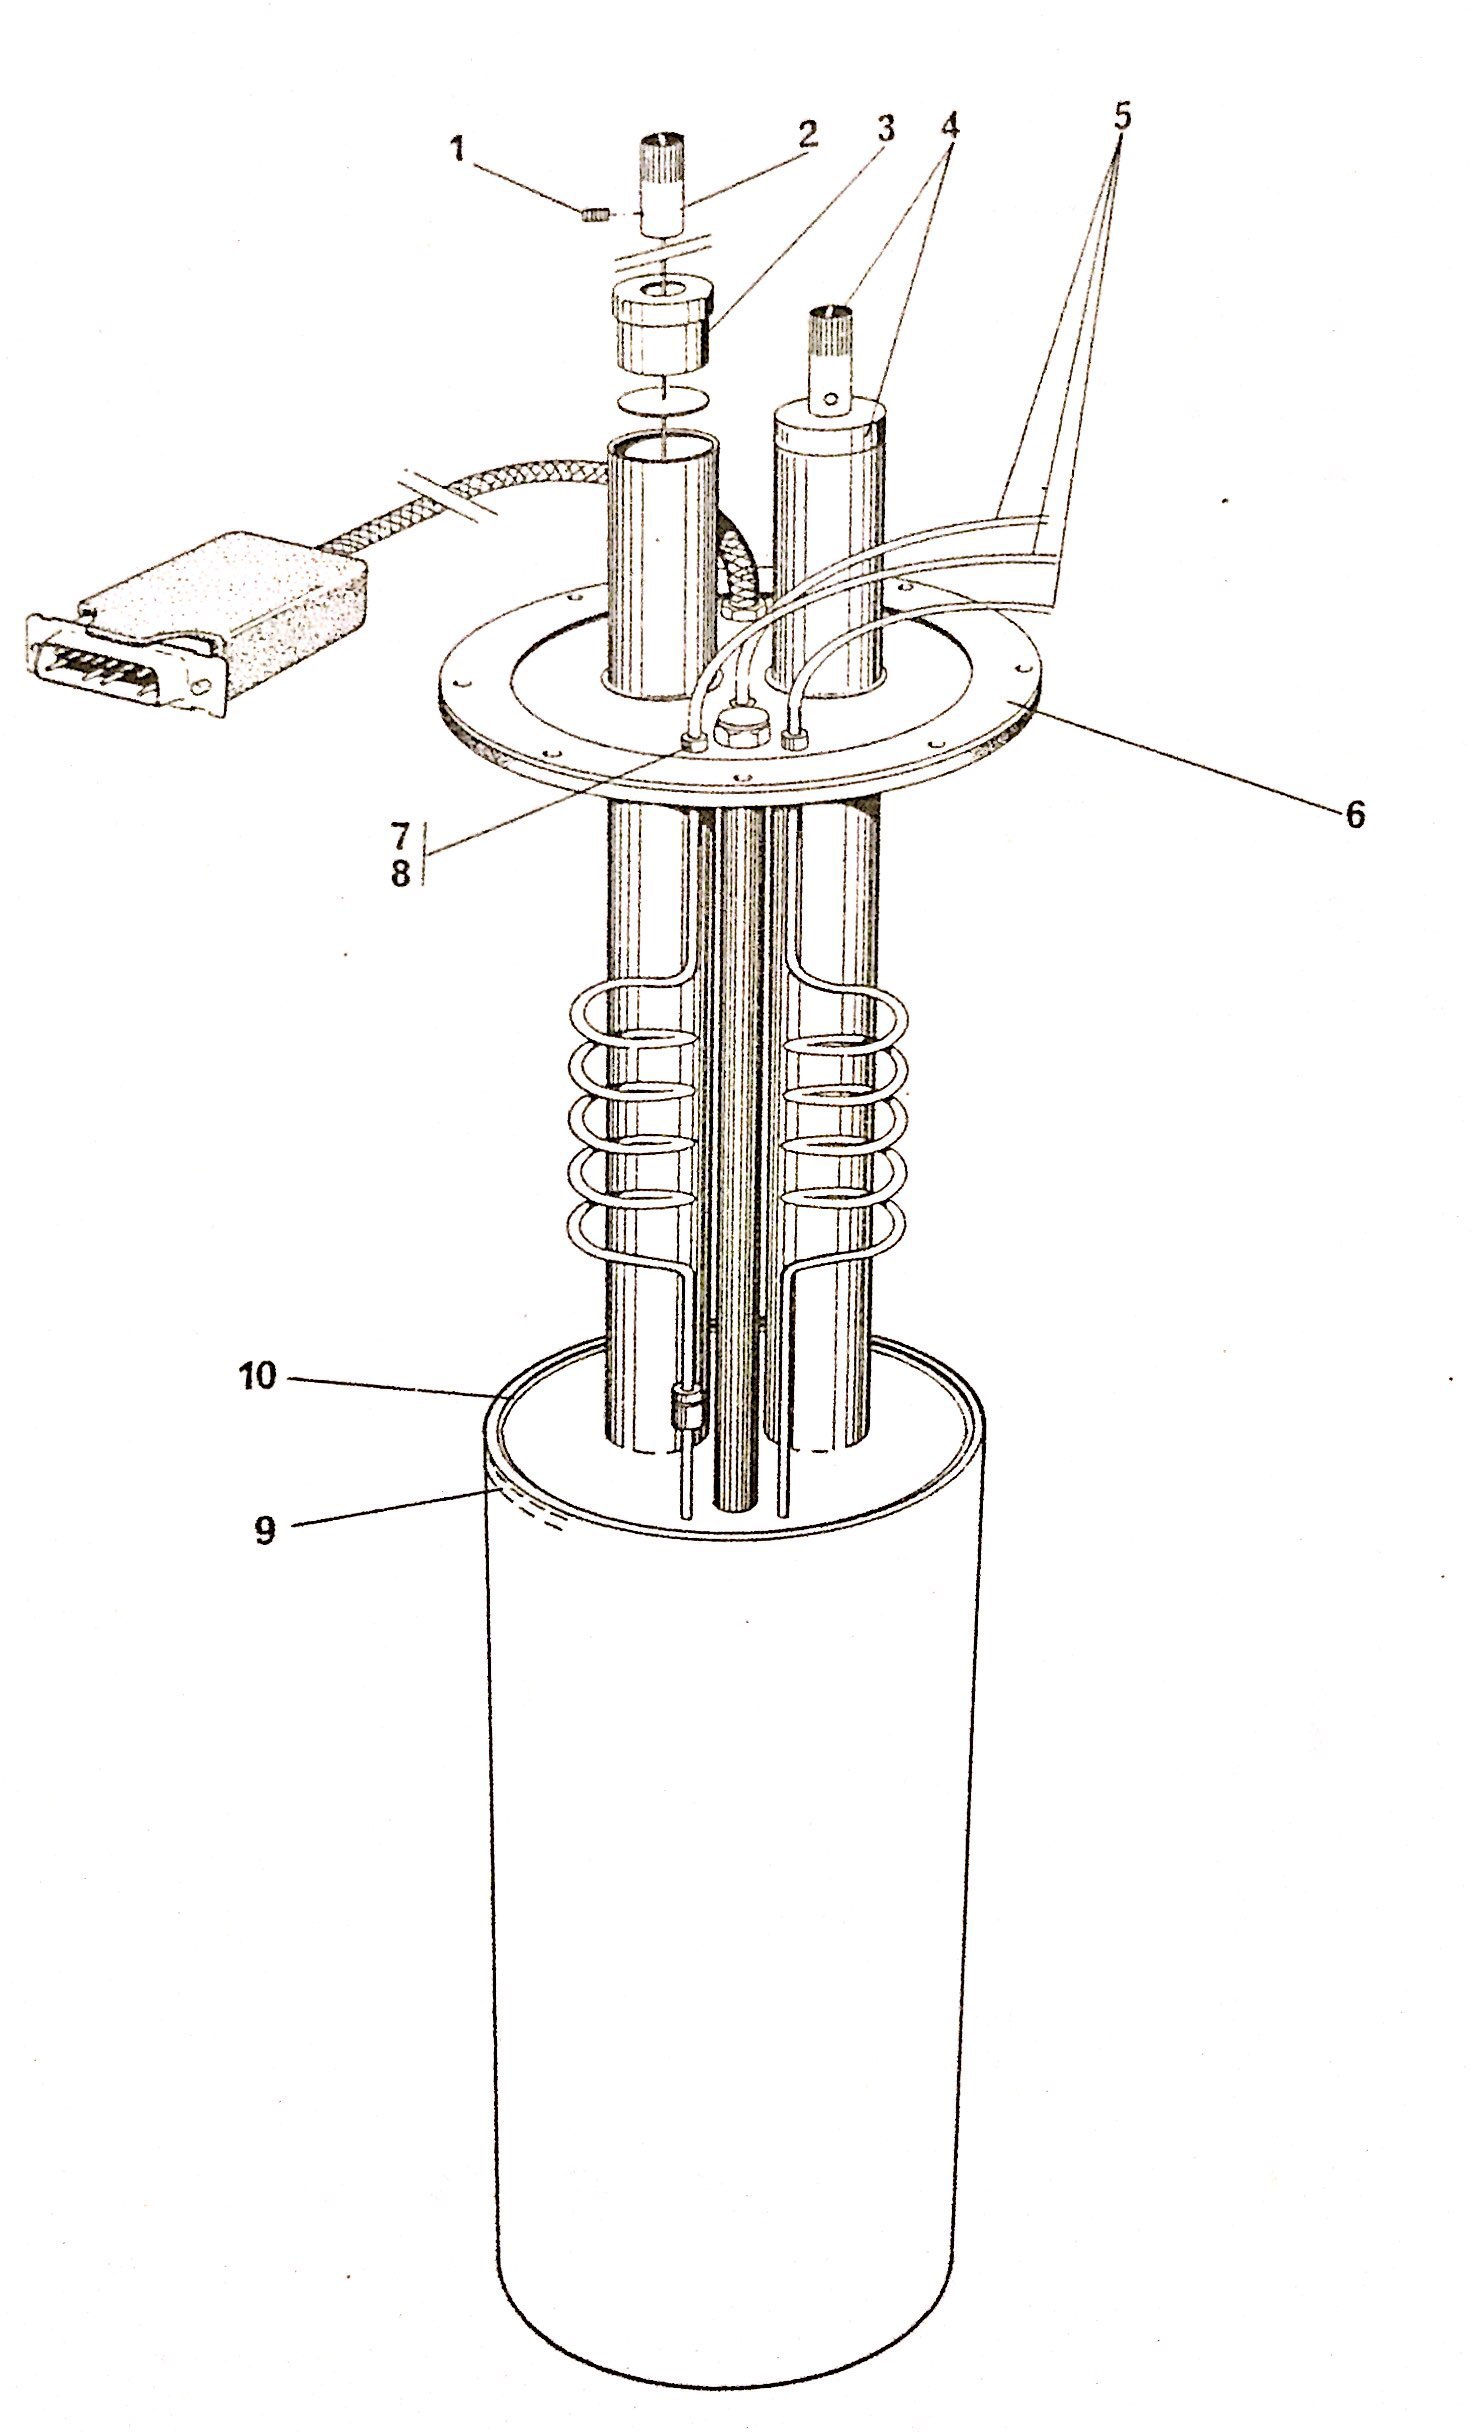
\includegraphics[width=\textwidth]{Figures/images_3.jpg}
%			\caption{Celda de medición.}
%			\label{fig:celda}
%		\end{subfigure}
%		\caption{Componentes exteriores del equipo y partes de los sistemas del calorímetro \cite{Suurkuusk}.}
%		\label{fig:partes}
%	\end{figure}
%	Usando esta información se llevará a cabo el ensamble del calorímetro así como las conexiones eléctricas.	A nivel electrónico, la liberación o absorción de energía térmica se mide usando una celda Peltier, las cuales tienen una respuesta proporcional en voltaje, de esta forma se obtiene una señal eléctrica a partir de pequeñas variaciones de temperatura en la celda de reacción. La señal eléctrica es procesada por el sistema digital del instrumento \cite{Suurkuusk}. De esta forma y siguiendo las instrucciones es posible realizar una calibración eléctrica del sistema.
%	
%	La calibración química puede realizarse de distintas maneras. En principio cualquier reacción que pueda ser llevada a cabo en un calorímetro, con condiciones controladas y cuyas propiedades termodinámicas sean bien conocidas, puede ser usada como una reacción de calibración \cite{wadso2001standards}. Sin embargo es recomendable que los reactivos involucrados en estas reacciones no requieran de algún tipo de purificación que pueda alterar el análisis \cite{wadso2001standards}.
%	
%	Se propone realizar una calorimetría de titulación como método de calibración química, lo anterior es importante porque una calibración eléctrica puede dar lugar a distribuciones de temperatura distintas en la celda de reacción, o generar patrones de flujo de calor distintos a una reacción química, esto puede generar errores sistemáticos en las medidas realizadas \cite{wadso2001standards}. La titulación es una técnica importante en la medida que permite la determinación simultánea de la entalpía molar y la constante de equilibrio de la reacción, por lo cual también se obtienen el cambio en la energía estándar de Gibbs y el cambio en la entropía estándar \cite{wadso2001standards}. 
%	
%	Para esta calibración es necesario contar con soluciones acuosas de cloruro de bario (\ce{BaCl2}) y éter 18-corona-6 (\ce{[C2H4O]6}) \cite{tellinghuisen2007optimizing, mizoue2004calorimetric, wadso2001standards}. La reacción de acomplejamiento es 1:1, de la siguiente forma:
%	\begin{equation}
%		\ce{Ba^{2+}(ac) + [C2H4O]6(ac) -> Ba^{2+}.[C2H4O]6(ac)}
%	\end{equation}
%	
%	Dichas soluciones deben encontrarse en el rango de concentraciones de 1 mM a 10 mM para el éter y 10 mM hasta 100 mM para el cloruro de bario. Dentro de este rango, existe evidencia experimental que muestra que no hay una variación significativa de las cantidades termodinámicas medidas \cite{wadso2001standards, mizoue2004calorimetric}. Considerando el volumen de las celdas con las que cuenta el equipo, se propone usar 1.5 mL de la solución de éter. Las soluciones deben ser desgasificadas y  termostatadas a 25 $^\circ$C, con el objetivo de limitar el error experimental introducido por diferencias de temperatura causadas por burbujas \cite{mizoue2004calorimetric, tellinghuisen2007optimizing, duff2011isothermal}. 
%	
%	En el calorímetro el ba\~no debe encontrarse a 25 $^\circ$C y deben usarse dos de las cuatro celdas disponibles. La primera se considera como referencia y debe contener al disolvente únicamente, en este caso 1.5 mL de agua \cite{Suurkuusk}. En la segunda se adiciona el mismo volumen de la solución de éter, una vez la línea base del calorímetro se encuentra estable, se adicionan una a una 30 alícuotas de la solución de cloruro de bario, con tiempos entre inyección mayores a $\tau = 6$ minutos, tanto a la celda de referencia como a la de reacción \cite{mizoue2004calorimetric, duff2011isothermal}. Cada inyección modifica la temperatura de la celda respecto a la referencia, razón por la cual las termopilas Peltier, deberán compensarla, la energía requerida por las celdas se cuantifica en función del tiempo, esto da lugar a una gráfica de potencia en función del tiempo \cite{duff2011isothermal}. Para cada inyección, es posible calcular el cambio en la energía integrando la potencia usada por el sistema. La gráfica de los cambios energéticos en función de la fracción molar (\ce{[Ba^{2+}]}/[éter]) permite obtener  las propiedades termodinámicas \cite{duff2011isothermal, mizoue2004calorimetric}. La diferencia entre el valor mínimo de la isotérma y la línea base de esta corresponde con la entalpía molar estándar $\Delta H_m$. La derivada de la isotérma en el punto equimolar, da lugar a la constante de afinidad $K_a$. Finalmente con esta es posible determinar los cambios en la energía libre de Gibbs y la entropía.
%	
%	\begin{equation}
%		\Delta G_m = -RT\ln K_a = \Delta H_m - T\Delta S_m
%	\end{equation}
%	
%	Para determinar la capacidad calorífica es necesario realizar el mismo experimento a distintas temperaturas, dado que:
%	\begin{equation}
%		C_{p, m} = \left(\dfrac{\partial H_m}{\partial T}\right)_p
%	\end{equation}
%	
%	En el caso de esta titulación los valores reportados por IUPAC corresponden con \cite{wadso2001standards}:
%	\begin{itemize}
%		\item $\Delta H_m = -(31.42 \pm 0.20)$ kJ mol$^{-1}$
%		\item $K_a = (5.90 \pm 0.20)\times10^3$ mM
%		\item $C_{p,m} = 126$ J K$^{-1}$ mol$^{-1}$
%	\end{itemize}
%\include{Chapters/Chapter2} 
%\include{Chapters/Chapter3}
%\include{Chapters/Chapter4} 
%\include{Chapters/Chapter5} 

%----------------------------------------------------------------------------------------
%	THESIS CONTENT - APPENDICES
%----------------------------------------------------------------------------------------

%\appendix % Cue to tell LaTeX that the following "chapters" are Appendices

% Include the appendices of the thesis as separate files from the Appendices folder
% Uncomment the lines as you write the Appendices

%\include{Appendices/AppendixA}
%\include{Appendices/AppendixB}
%\include{Appendices/AppendixC}

%----------------------------------------------------------------------------------------
%	BIBLIOGRAPHY
%----------------------------------------------------------------------------------------

\printbibliography[heading=bibintoc, title={Referencias}]

%----------------------------------------------------------------------------------------

\end{document}  
